\section{Theorie}
\subsection{Wireless Local Area Network (WLAN)} 
\subsubsection{Beschreibung}
Als lokales Funknetz ist WLAN weit verbreitet. WLAN ist eine Abkürzung für Wireless-Local-Area-Netzwerk, in deutsch ein Drahtloses-Lokales-Areal-Network. Die Idee der lokalen Funkkommunikation war, dass in Büros mit mobilen Geräten wie Laptops eine kabellose Verbindung zum Internet hergestellt werden kann. Damit die Anbindung an das standardisierte LAN nicht in jedem Büro unterschiedliche Eigenschaften benötigt, wurde vom IEEE-Komitee entschieden ein Standard einzuführen, das Komitee entwickelte somit den 802.11 Standard für die drahtlosen Verbindungen. IEEE-802.11 Systeme nutzen unlizenzierte Frequenzbänder Bänder wie z.B. 902-928 MHz oder 2.4 - 2.5 GHz. Sämtliche Geräte dürfen dieses Spektrum nutzen, vorausgesetzt sie begrenzen ihre Sendeleistung, damit mehrere Geräte nebeneinander betrieben werden können. IEEE-802.11 Netze bestehen aus Clients wie Laptops und Smartphones sowie einer Infrastruktur, Zugangspunkt AP (Access Point), welcher im Gebäude installiert ist. Der AP ist die Schnittstelle zum verkabelten Netz und ist im Privathaushalt oft direkt im Modem nebst dem Router integriert, siehe Abbildung \ref{pic: IEEE802.11}.


 \begin{figure}[H]
	\centering
	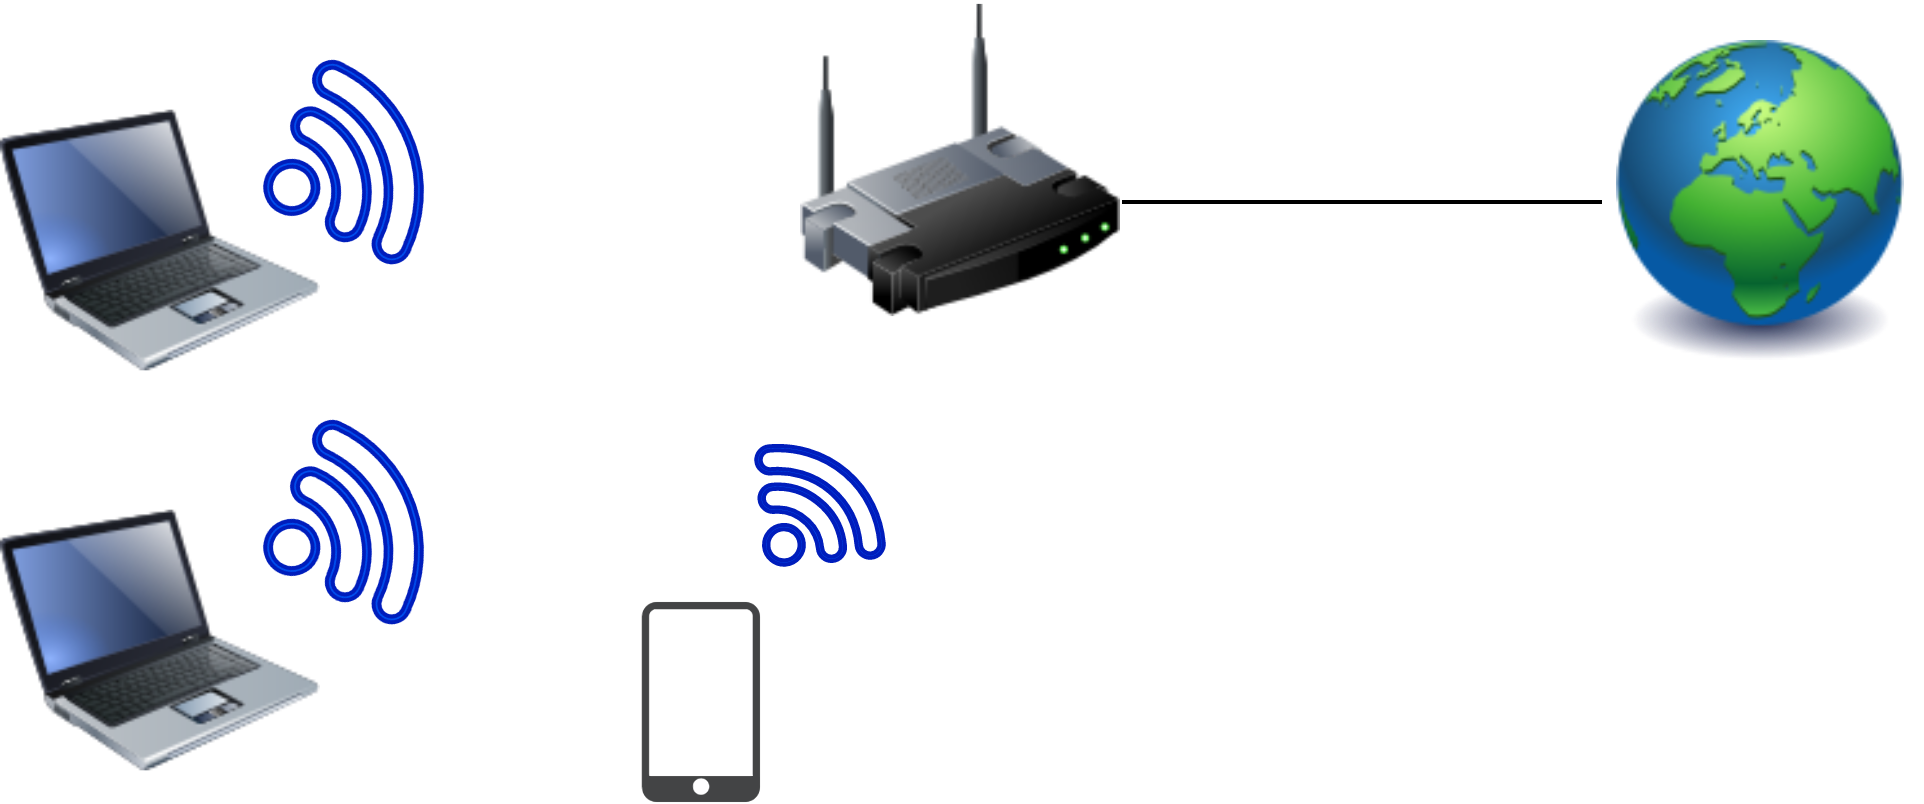
\includegraphics[width=\textwidth]{graphics/IEEE80211.png}
	\caption{Übersicht IEEE 802.11} 	
	\label{pic: IEEE802.11}
\end{figure} 
\subsubsection{Datenrate}
Der IEEE 802.11 Standard definierte 1997 ein drahtloses LAN, das entweder 1 Mbit/s oder 2 Mbit/s sendete und entweder Frequenzen wechselte oder das Signal über das erlaubte Spektrum verstreute. Die Funkverbindung wurde weiterentwickelt, so dass die Geschwindigkeit zunahm, in der nachfolgenden Tabelle ist eine Übersicht.
\begin{table}[H]
	\centering
	\begin{tabular}{|c|c|c|}
		\hline 
		Standard & Übertragungsleistung & Modulation \\ 
		\hline 
		IEEE-802.11b & 11Mbit/s & Frequenzspreizung \\ 
		\hline 
		IEEE-802.11a/g & 54Mbit/s & OFDM \\ 
		\hline 
		IEEE-802.11n & 450Mbit/s & Mehrerere Frequenzbänder \\ 
		\hline 
	\end{tabular} 
\caption{IEEE 802.11 Standarts \cite{wetherall_computernetzwerke_2012}}
\label{tab: IEEE802.11Standartds}
\end{table}
Das OFDM-Schema, Orthogonal Frequency Division Multiplexing, verwendet mehrere Trägerfrequenzen. Mehrere eng beieinanderliegende orthogonale Hilfsträgersignale mit überlappende Spektren übertragen Daten parallel.

\subsubsection{Sicherheit}

Die kabellosen Übertragungen sind Broadcast-Verbindungen, daher besteht das Problem, dass Informationspakete abgefangen werden können. Um dies zu verhindern ist im IEEE  802.11 Standard das Verschlüsselungsschema, WEP (Wired Equivalent Privacy) enthalten. Das WEP wurde durch WPA (WiFi Protected Access) ersetzt, und schliesslich wurde WPA durch WPA2 ersetzt. Im Juni 2018 wurde von Wi-Fi Alliance WPA3 vorgestellt, die nächste Generation der WiFi Sicherheit.\\
\\
\subsubsection{Funktion WPA2}

Die WPA2 Verschlüsselung wird in zwei verschiedenen Szenarien verwendet.\\
Ein Unternehmen hat ein Authentifizierungsserver mit Benutzernamen und Kennwortdatenbank eingerichtet, mit dem festgelegt wird ab ein drahtloser Client auf das Netz zugreifen darf. In diesem Fall verwenden Clients Standardprotokolle, um sich zu authentifizieren.
Im zweiten Szenario haben alle Clients ein gemeinsames Passwort, die Verbindung wird ohne Authentifizierungsserver aufgebaut. Diese Methode wird oft in privaten Netzwerken angewendet. Der Hauptunterschied ist, dass beim Authentifizierungsserver jeder Client ein Schlüssel zur Datenverschlüsselung bekommt, beim gemeinsamen Passwort wird der Schlüssel bei jedem Client aus dem Passwort abgeleitet und ist daher weniger sicher.
Nach dem sich der Client mit dem Passwort ausgewiesen hat, geschieht ein 4-Pakete-Handshake, und somit werden weitere Schlüssel erstellt.  
\subsubsection{WPA2 im Vergleich zu WPA3}
Bei WPA3 gibt es wieder die 2 verschiedenen Betriebsarten.\\
WPA3-Personal bietet eine stabilere Kennwort basierte Authentifizierung, selbst wenn Benutzer Kennwörter ändern, SAE (Simultaneous Authentication of Equals), schützt den Benutzer stärker gegen Dritte, welche versuchen das Passwort zu erraten.\\
WPA3 Enterprise bietet kryptografischen Schutz mit der Stärke von 192 Bit, somit geeignet für sensible Daten von einem Finanzinstitut \cite{noauthor_wi-fi_nodate}.























\newpage
\subsection{Message Queuing Telemetry Transport (MQTT)}
\subsubsection{Beschreibung}
MQTT ist ein Nachrichtentransport Protokoll, mittels Client werden Nachrichten veröffentlicht sprich abonniert und mit dem MQTT-Broker verwaltet. Anwendung findet MQTT im Bereich in eingeschränkten Umgebungen, wie Kommunikation von Maschine zu Maschine (M2M) und Internet der Dinge (IoT). Das Protokoll läuft über TCP/IP oder über andere Netzwerkprotokolle, welche verlustfreie bidirektionale Verbindungen bieten \cite{noauthor_mqtt-v5.0.pdf_nodate}. 

\subsubsection{Geschichte}
MQTT wurde 1999 von dr.Andy Stanford-Clark von IBM und Arlen Nipper von Arcom erfunden. Seit 2013 ist MQTT über die nicht gewinnorientierte Organisation OASIS als Protokoll des Internet der Dinge standardisiert \cite{noauthor_mqtt-v5.0.pdf_nodate}. .
\subsubsection{Überischt}
 \begin{figure}[H]
 	\centering
 	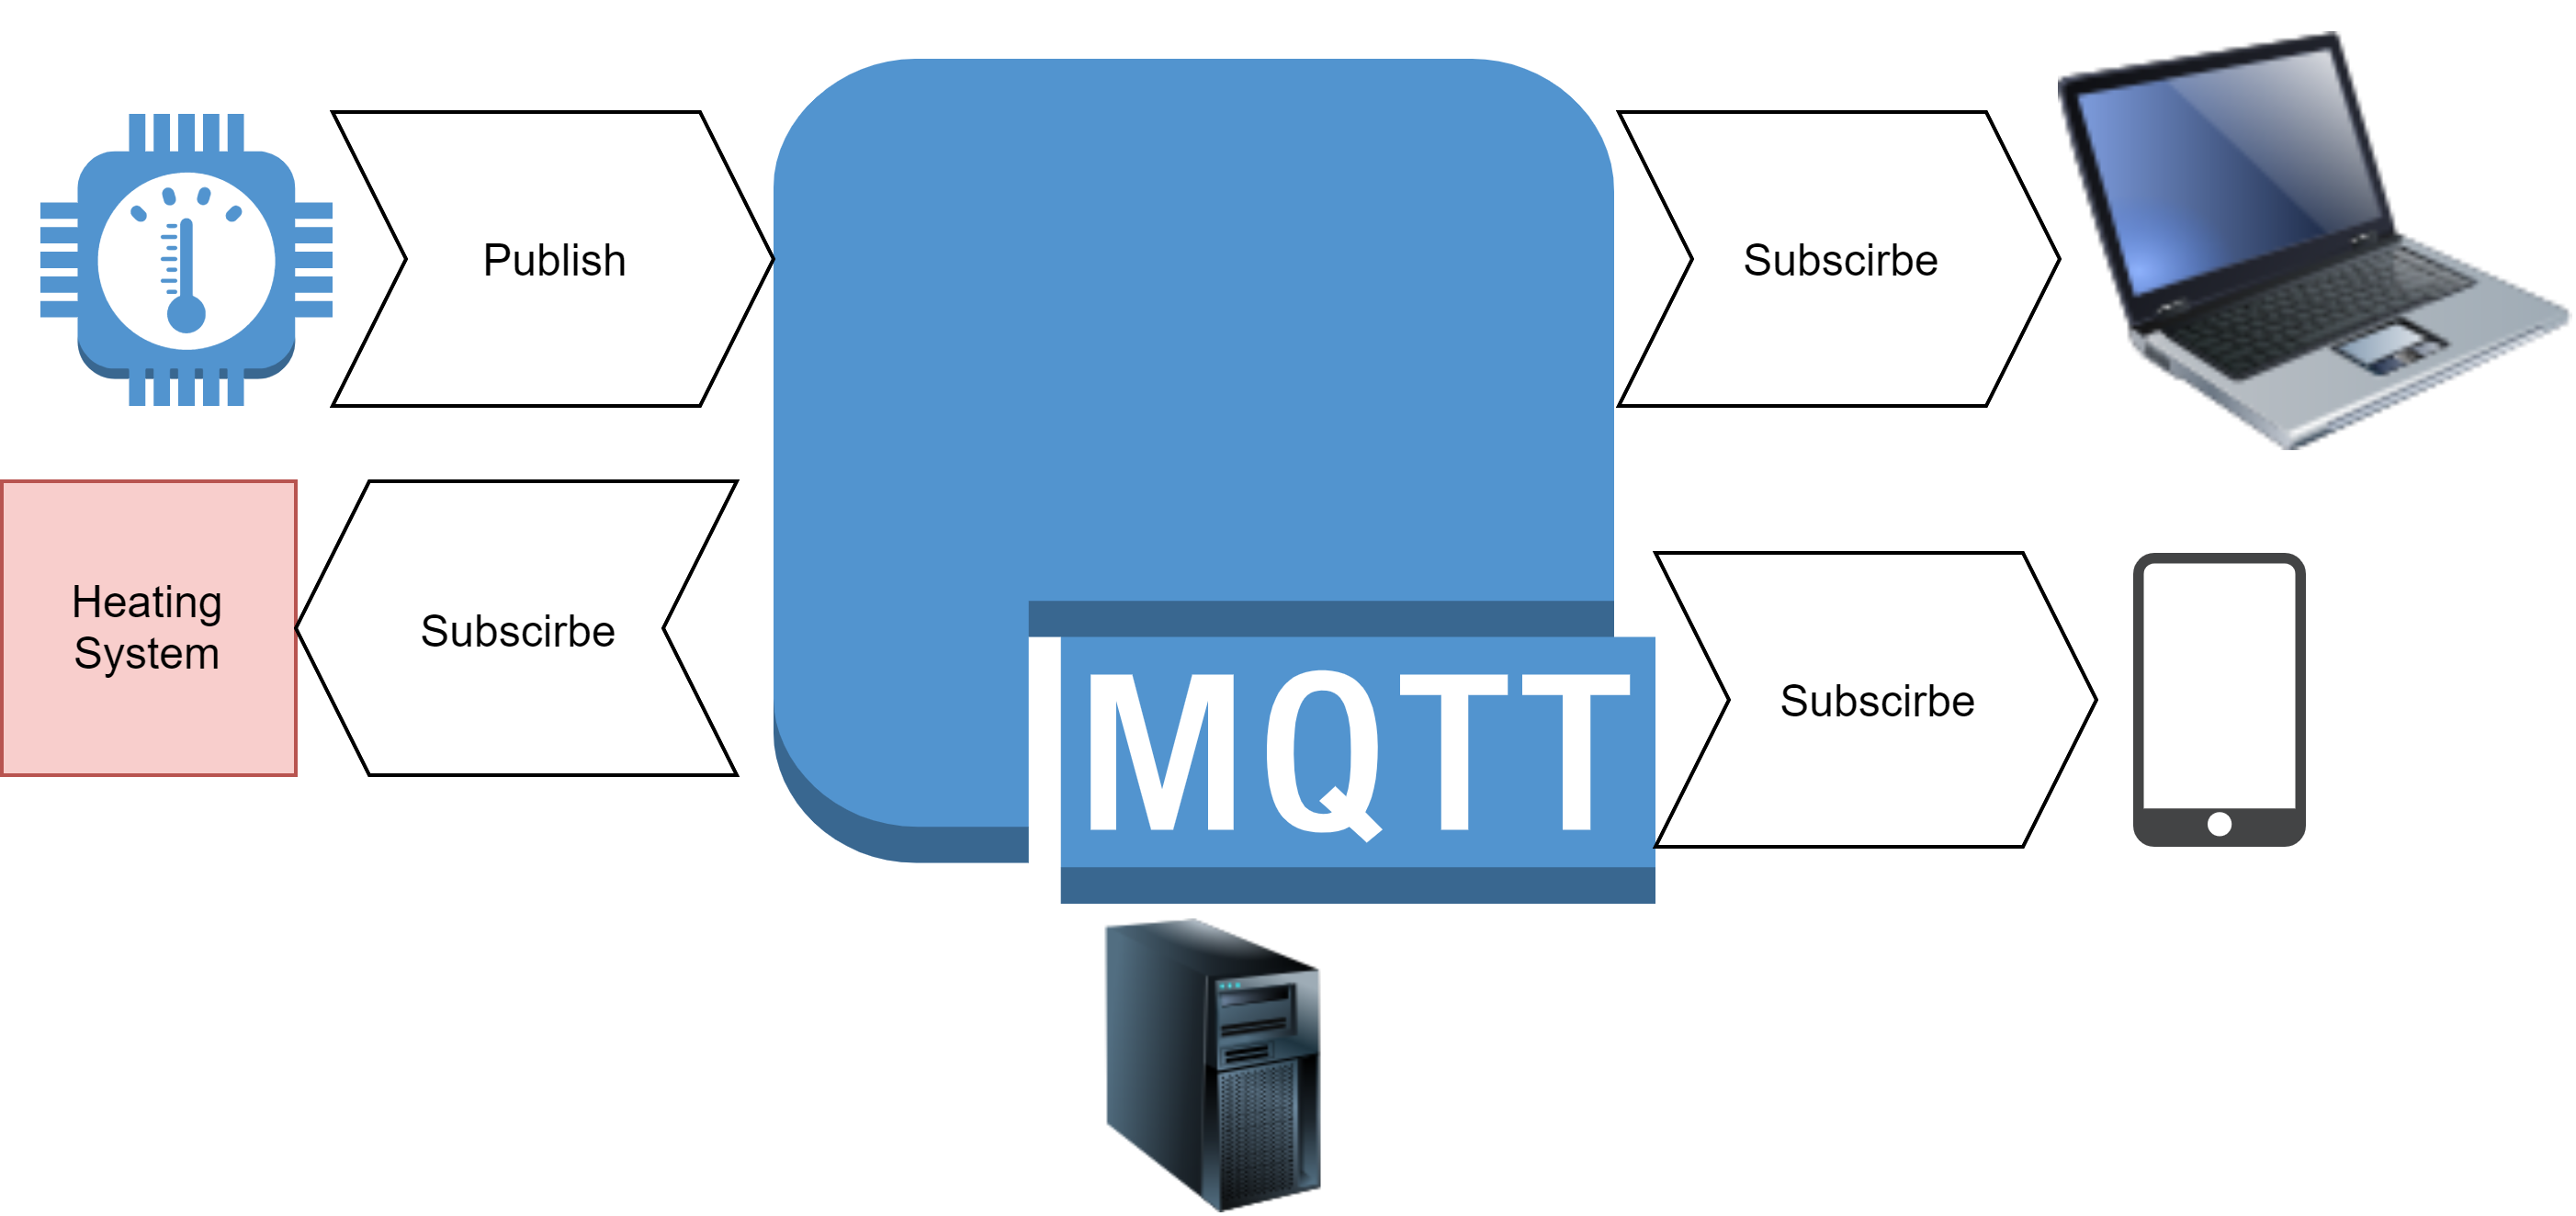
\includegraphics[width=\textwidth]{graphics/OverviewMQTT.PNG}
 	\caption{Übersicht MQTT} 	
 	\label{pic: OverMQTT}
 \end{figure} 
In der Abbildung \ref{pic: OverMQTT} werden Daten von einem Thermostat veröffentlicht. Ein Heizsystem, ein Notebook und ein Smartphone haben die Daten abonniert und der MQTT-Broker verwaltet die Nachrichten. 

\subsubsection{MQTT-Server (Broker)}
Der MQTT-Server ist ein Programm oder Gerät, welches als Vermittler zwischen Clients dient und wird auch als MQTT-Broker bezeichnet. Der Broker nimmt Netzwerkverbindungen von Clients an, empfängt so die Nachrichten von Clients und gibt diese Nachrichten an jene Clients weiter, welche ein Abonnement abgeschlossen haben.

\subsubsection{Client}
Ein Client ist ein Programm oder Gerät, welches MQTT verwendet. Dieser baut eine Verbindung zum Broker auf. Der Client veröffentlicht Nachrichten mit einem Topic und einer Payload. Ist ein Client an bestimmten Daten interessiert abonniert er diesen Topic und empfängt somit die Payload.
 
\subsubsection{Eigenschaften MQTT Broker}
Veröffentlichen, abonnieren oder  Publish/Subscribe kann in Form von One-to-many Nachrichten verwendet werden.\\
MQTT benötigt wenig Zusatzinformationen beim Transport und minimiert so die Protokoll Austausche, somit wird die Belastung des Netzwerkverkehrs minimiert.\\
Es gibt ein Mechanismus zur Benachrichtigung interessierter Parteien, wenn eine Unterbrechung einer Verbindung auftritt.\\
Für die Nachrichten Zustellung gibt es drei Service Qualitäten \cite{steve_understanding_nodate}:\\
\begin{itemize}
	\item Einmal übertragen, in diesem Fall wird die Nachricht, mit den besten Bemühungen der Betriebsumgebung, übermittelt.\\
		\item Mindestens einmal übertragen, wobei sichergestellt wird, dass die Nachricht ankommt, aber Duplikate auftreten können.\\
	\item Exakt einmal übermitteln, in diesem Fall wird sichergestellt, dass die Nachricht genau einmal ankommt.
\end{itemize}

\subsection{Mqtt Paket Struktur}
MQTT ist ein binärbasiertes Protokoll, bei dem die Steuerelemente Binäre Bytes sind, jedem Befehl ist eine Bestätigung zugeordnet.

\begin{figure}[H]
	\centering
	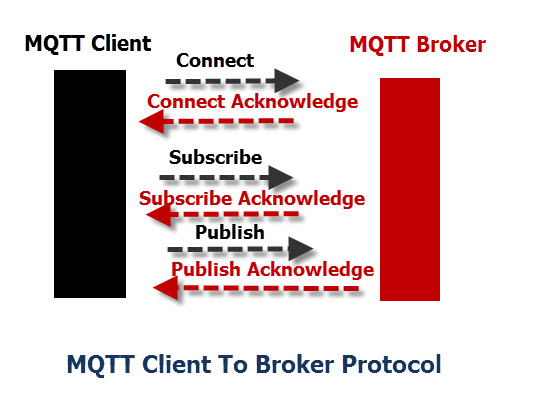
\includegraphics[width=0.75\textwidth]{graphics/MQTTProtocolCommands.jpg}
	\caption{Protokoll Verbindung Client zu Broker \cite{steve_understanding_nodate}} 	
	\label{pic: MQTTBrokerToClient}
\end{figure} 

Topic Namen, Client-ID und Benutzernamen werden als UTF-8-Strings kodiert. Die Payload sind binäre Daten, der Inhalt wie das Format sind anwendungsspezifisch. Das MQTT-Packet besteht aus einem festen 2 Byte-Header und der Payload bei bedarf kann noch ein variablen Header hinzugefügt werden.

\begin{figure}[H]
	\centering
	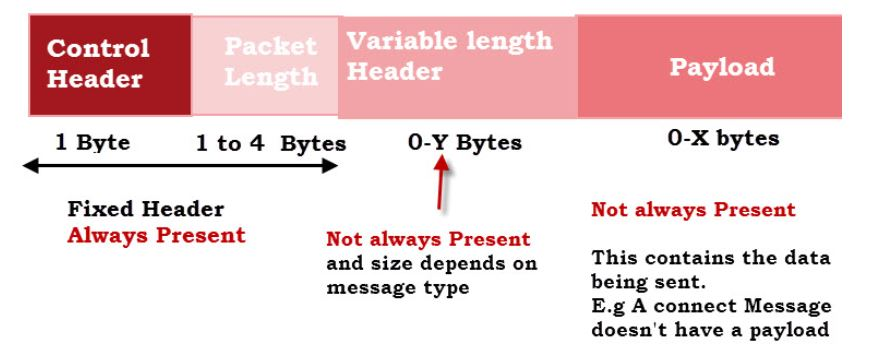
\includegraphics[width=0.75\textwidth]{graphics/MQTT-Standard-Packet.jpg}
	\caption{Standard MQTT Paket Struktur \cite{steve_understanding_nodate}} 	
	\label{pic: Struktur}
\end{figure} 

Es gibt 3 Grundlegende Paket Formate

\begin{itemize}
	\item Fester Header (Steuerfeld und Länge)\\
	\item Fester Header (Steuerfeld und Länge) und variable Payload\\
	\item Fester Header (Steuerfeld und Länge) variabler Header und variable Payload\\
\end{itemize}

Die Mindestlänge eines Pakets beträgt 1 Bit. 

Die maximale Paket grösse beträgt 256 MB.

Das Steuerfeld ist das erste Byte des Headers es ist in zwei 4-Bit Felder unterteilt und enthält Protokollbefehle wie auch antworten.